%% LaTeX-Beamer template for KIT design
%% by Erik Burger, Christian Hammer
%% title picture by Klaus Krogmann
%%
%% version 2.4
%%
%% mostly compatible to KIT corporate design v2.0
%% http://intranet.kit.edu/gestaltungsrichtlinien.php
%%
%% Problems, bugs and comments to
%% burger@kit.edu

%% Class options
%%   aspect ratio options: 
%%   -- 16:9 (default)
%%   -- 4:3
%%   language options: 
%%   -- en (default)
%%   -- de
%%   position of navigation bar:
%%   -- navbarinline (default): bottom of the white canvas
%%   -- navbarinfooter : more compressed variant inside the footer
%%   -- navbarside : side bar at the left of the white canvas
%%   -- navbaroff : none
%% example: \documentclass[16:9,de,navbarinfooter]{sdqbeamer}
\documentclass[16:9,en,navbarinfooter]{sdqbeamer}

%% \documentclass{sdqbeamer} 

%% TITLE PICTURE

% if a custom picture is to be used on the title page, copy it into the 'logos'
% directory, in the line below, replace 'myimage' with the 
% filename (without extension) and uncomment the following line
% (picture proportions: 63 : 20 for standard, 169 : 40 for wide
% *.eps format if you use latex+dvips+ps2pdf, 
% *.jpg/*.png/*.pdf if you use pdflatex)

% \titleimage{myimage}

%% GROUP LOGO 

% for a custom group logo, copy your file into the 'logos'
% directory, insert the filename in the line below and uncomment it

\grouplogo{irlalr}

% (*.eps format if you use latex+dvips+ps2pdf,
% *.jpg/*.png/*.pdf if you use pdflatex)

%% GROUP NAME

% for groups other than SDQ, please insert in the line below and uncomment it
% \groupname{My group}

% the presentation starts here 

\author{Caspar Friedrich Maximilian Nagy}

%% Title (and possibly subtitle) of the thesis
\title{Solving Real-World Robot Manipulation Tasks with Deep Reinforcement Learning}
\subtitle{Box Pushing with Motion Primitives on a real Panda Robot}

% Bibliography 
\usepackage{dsfont}
\usepackage{multimedia}
%\usepackage{media9}
\usepackage{booktabs}
\usepackage{longtable}
\usepackage{array}
\usepackage{algorithm}
\usepackage{algpseudocode}
\usepackage{pgfplots}
% \pgfplotsset{compat=1.15}
 \usepgfplotslibrary{groupplots}
\usepackage{subcaption}
\usepackage{pdflscape}
\usepackage{diagbox}
\usepackage{multicol}
\DeclareUnicodeCharacter{2212}{−}
\usepgfplotslibrary{groupplots,dateplot}
\usetikzlibrary{patterns,shapes.arrows}
\pgfplotsset{compat=newest}
\usepackage[citestyle=authoryear,bibstyle=numeric,hyperref,backend=biber%,style=verbose
]{biblatex}
\addbibresource{presentation.bib}
\bibhang1em
\usepackage{listings}
\begin{document}

%title page
\KITtitleframe{}

%table of
% \begin{frame}
%     \frametitle{Video Example}
%     Here is a video:
% 
%     %\movie[width=0.6\linewidth, height=0.45\linewidth, poster, showcontrols]{Click to play}{media/test.mp4}
%     \begin{columns}
%         \column{.6\textwidth}
%     \movie[width=\linewidth, height=0.5625\linewidth, poster, showcontrols]{Click to play}{media/test.mov}
%         \column{.4\textwidth}
%     \end{columns}
% \end{frame}

\begin{frame}
	\frametitle{Agenda}
	\vspace{1cm}
	\setcounter{tocdepth}{1}
	\tableofcontents
\end{frame}

\section{Motion Primitive-Based (Re-)Planning Policy (MP3)}
\begin{frame}{Motion Primitive-Based (Re-)Planning Policy (MP3)}

	\center
	\vspace{1cm}
	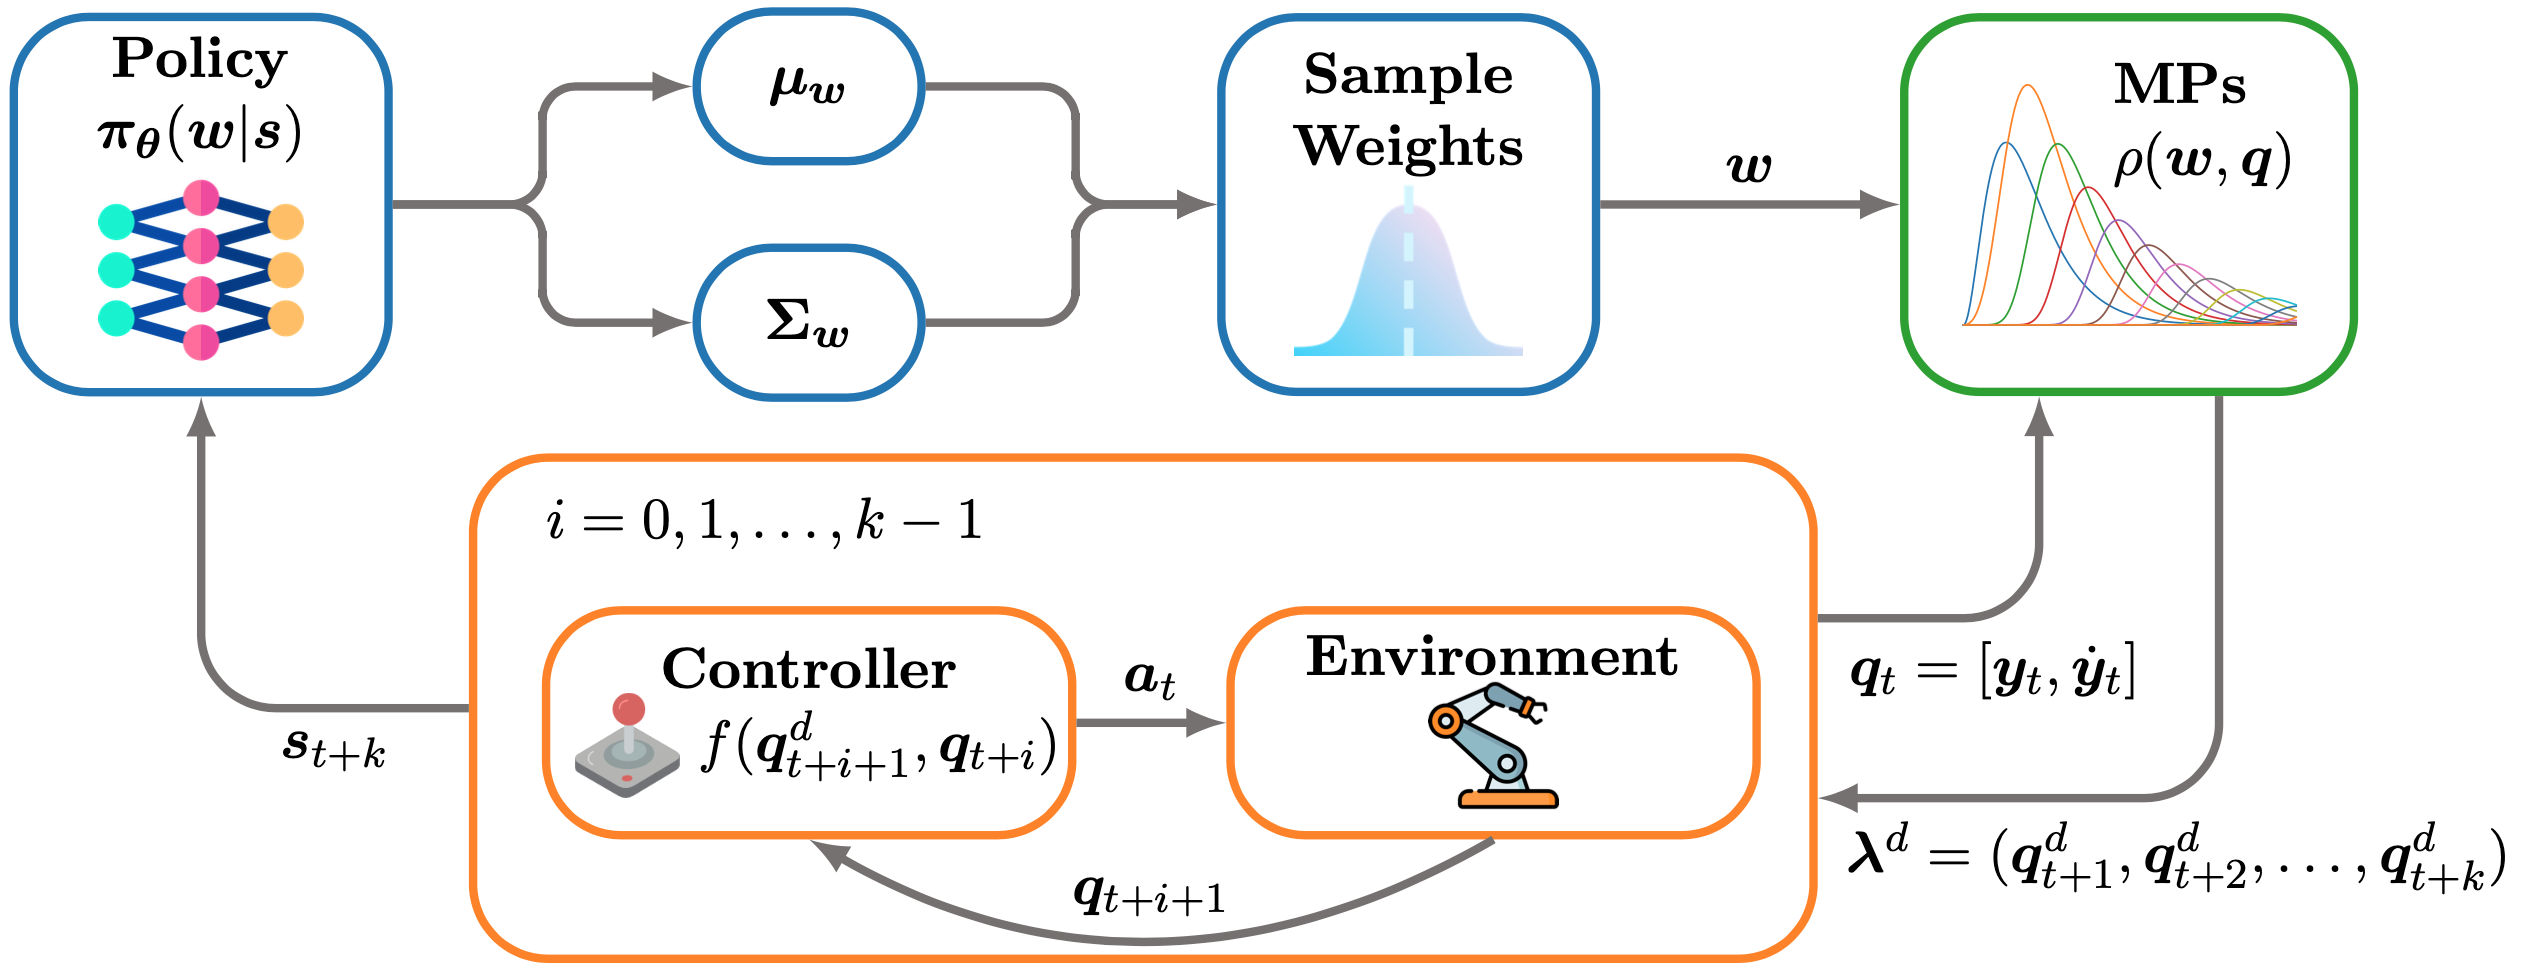
\includegraphics[width=.7\linewidth]{media/mp3.png}
	\begin{itemize}
		\item Blackbox and replanning variant
		\item Works with sparse, non-markovian rewards
		\item Generates smooth trajectories
		\item Trained on-policy using Trust Region Projection Layers (TRPL)
	\end{itemize}
\end{frame}

\subsection{MP3 in the Real World}
\begin{frame}{MP3 in the Real World}

	\center
	\vspace{1cm}
	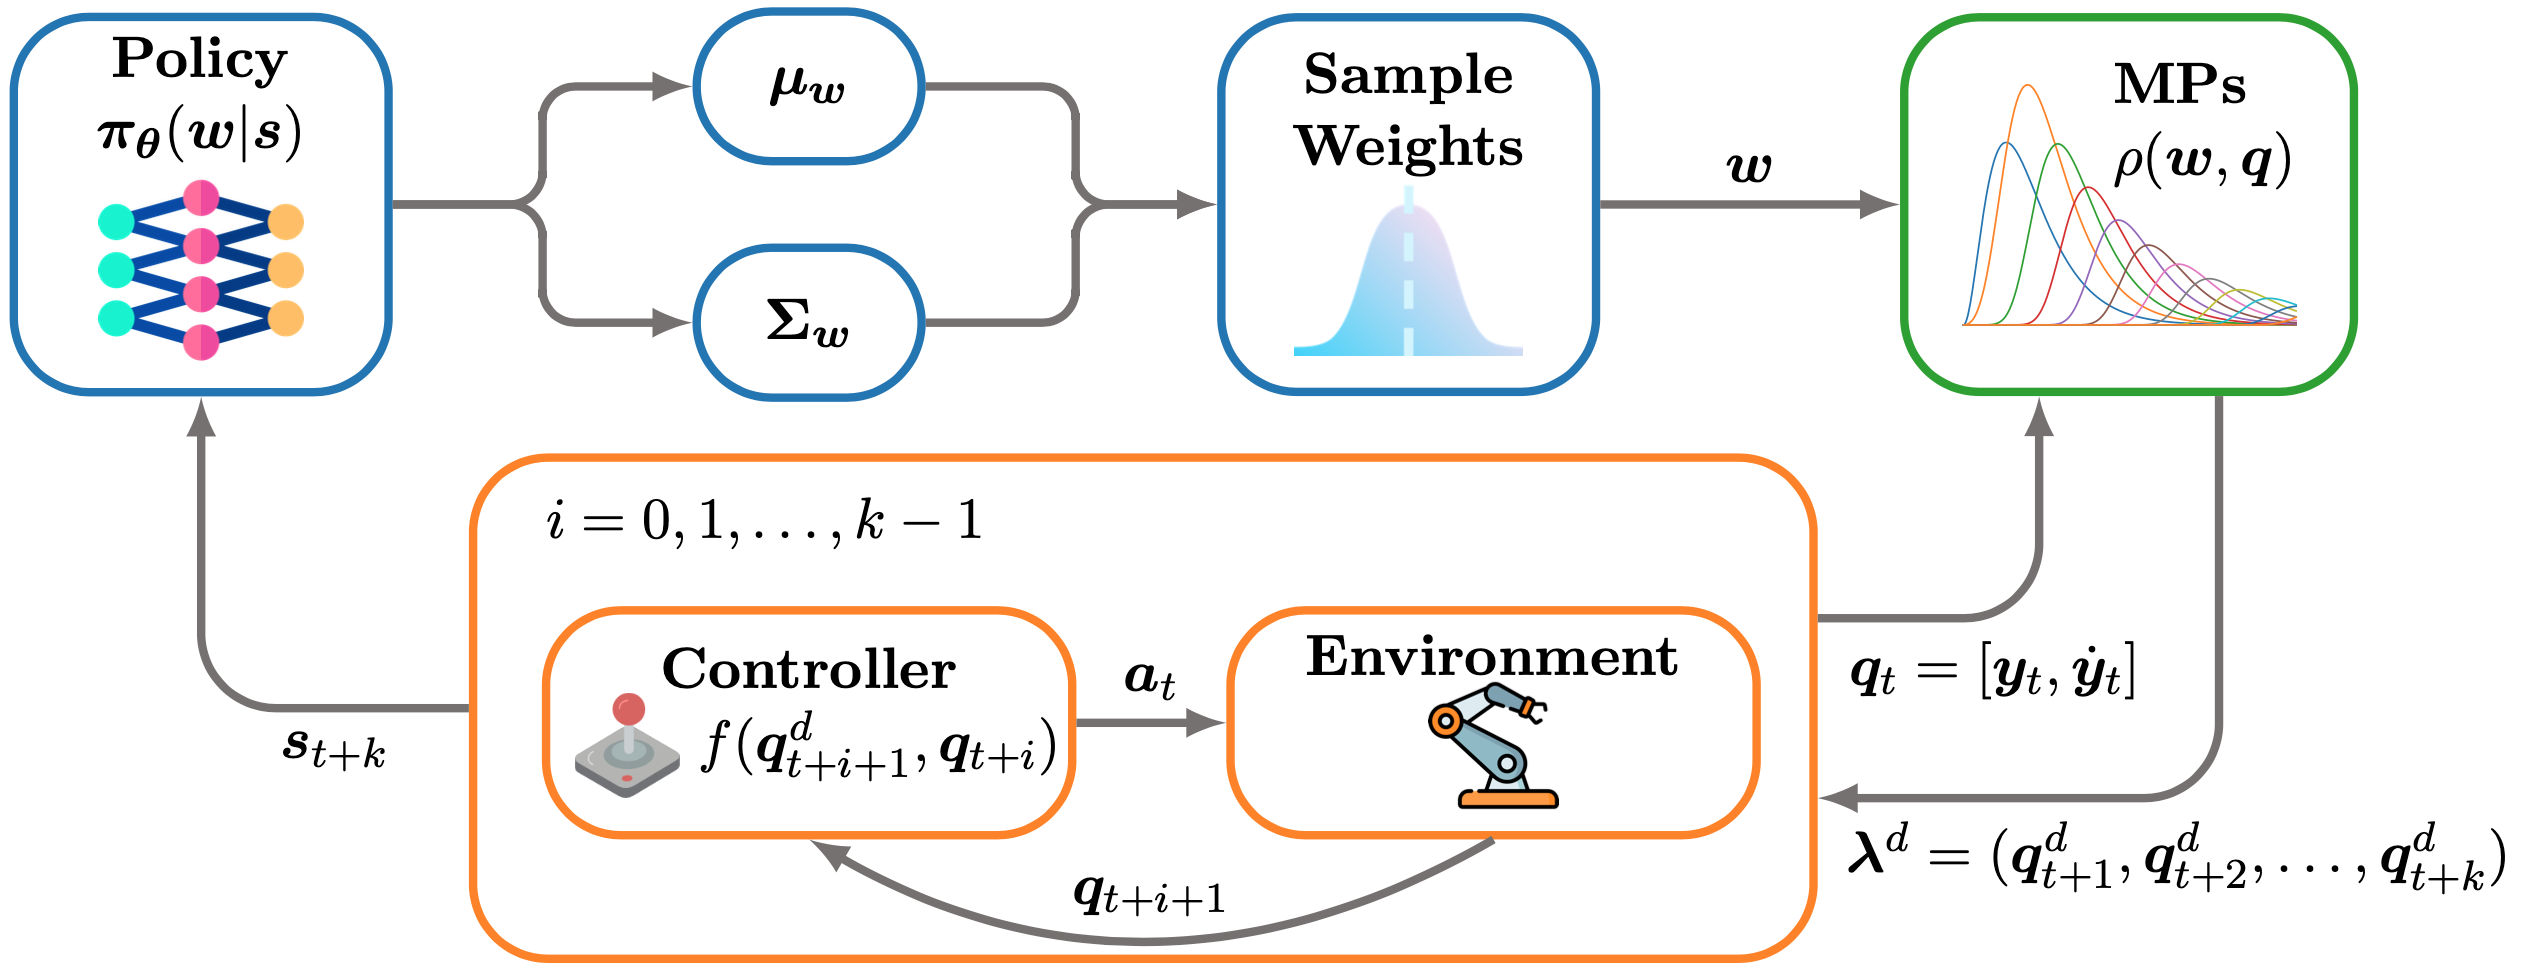
\includegraphics[width=.7\linewidth]{media/mp3.png}
	\begin{itemize}
		\item Contextual MPRL was never used on a real robot\dots will it work?
		\item How big is the sim2real gap?
		\item Do we need replanning?
		\item Is it better than step-based methods?
	\end{itemize}
\end{frame}

\subsection{Domain Randomization}


\begin{frame}{Box Pushing}
	\section{Box Pushing}

	\begin{columns}[t]
		\begin{column}{0.5\textwidth}
			\begin{itemize}
				\item Goal: Use a ``finger'' to push a box to a target pose
				      \begin{itemize}
					      \item Random start pose
					      \item Fixed target pose
				      \end{itemize}
			\end{itemize}
		\end{column}
		\begin{column}{0.5\textwidth}
			\begin{itemize}
				\item Challenges
				      \begin{itemize}
					      \item Underactuated system
					      \item Complex table-box interactions
					      \item Complex Panda kinematic
					      \item Trajectories must be safe and executable
				      \end{itemize}
			\end{itemize}
		\end{column}


	\end{columns}
	\center
	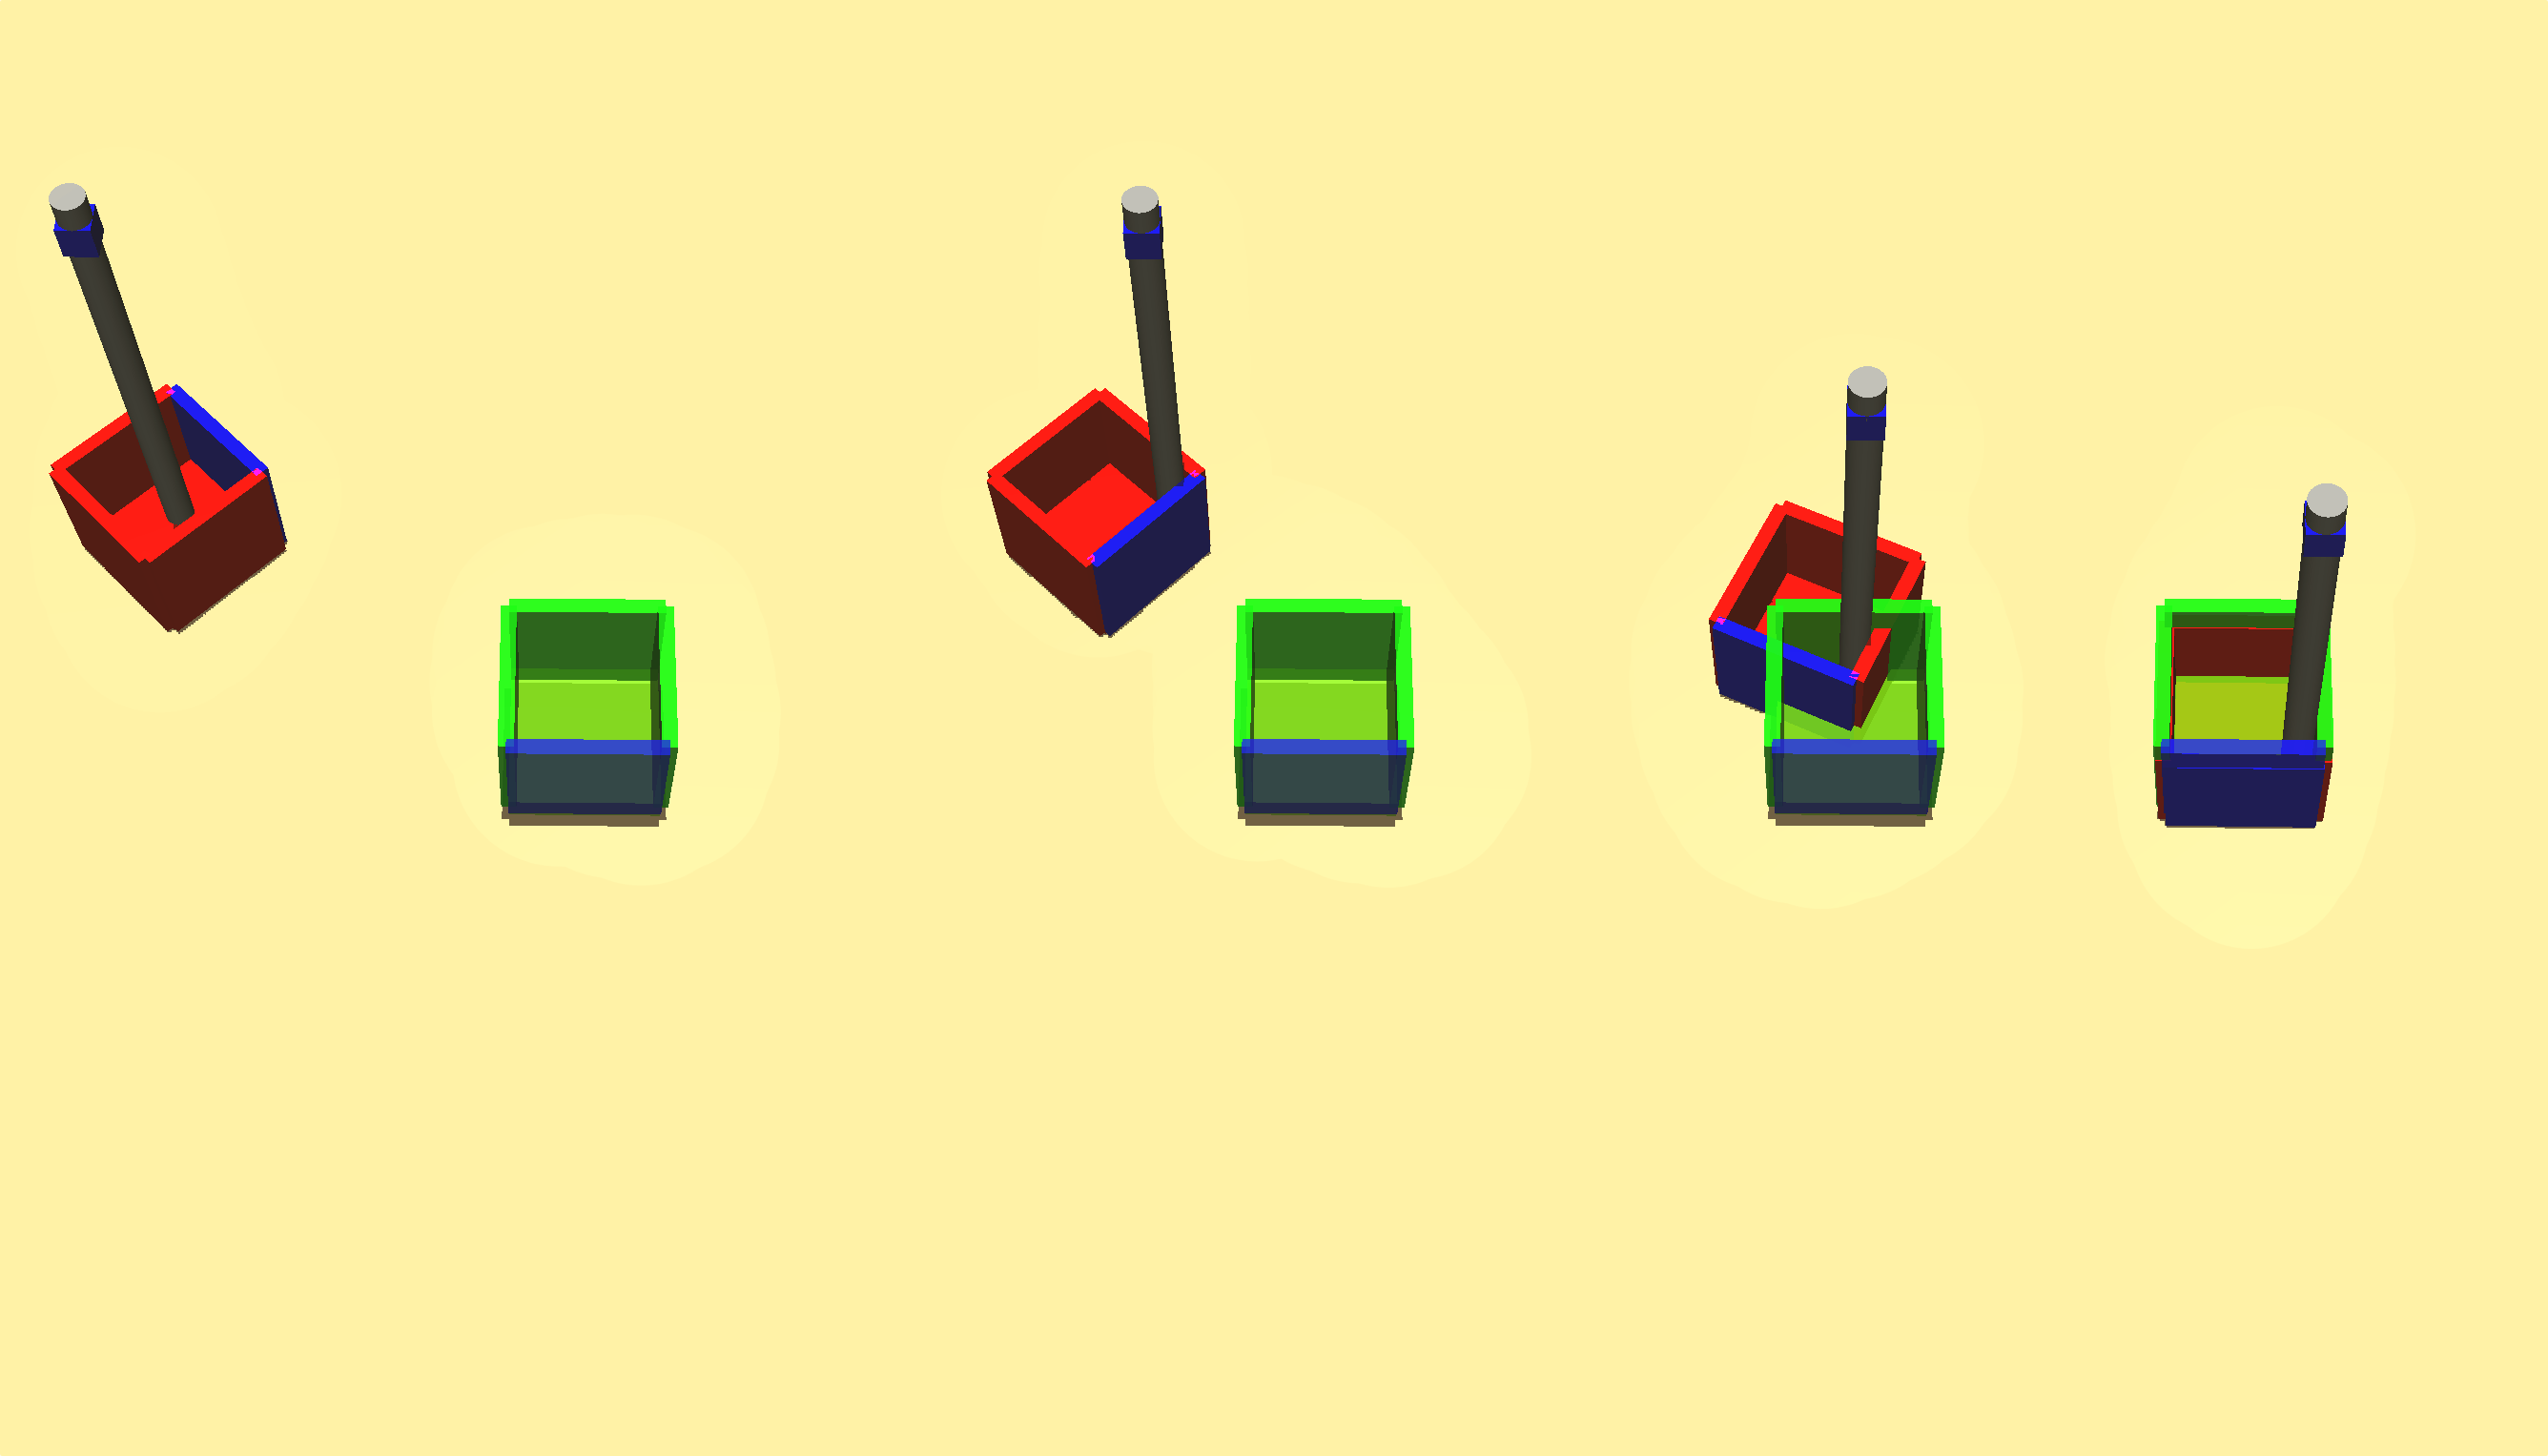
\includegraphics[height=3cm]{media/2dboxpushing.png}
	\vspace{.1cm}\\
	Box Pushing is a challenging benchmark problem for motion primitive reinforcement learning.
\end{frame}


\begin{frame}{How to get RL into the real World}
	\begin{itemize}
		\item Three important Approaches to Real-World RL
		      \begin{itemize}
			      \item Training on the Robot
			      \item Fine-Tuning
			      \item \textbf{Sim2Real}
		      \end{itemize}
		\item Sim2Real is a good fit for MP3 and the simplest to implement
		\item Problem: Sim2Real Gap
		\item Solution: Domain Randomization
		      \begin{itemize}
			      \item Friction $\mu \sim 0.43 \pm 0.1$ \quad (System Dynamics)
			      \item Box Position $x_\text{obs} \sim x \pm 5cm$ \quad (Observations)
			      \item Controller P-Gain $k_p \sim k_p^* \pm 68$ \quad (Actions)
		      \end{itemize}

	\end{itemize}

\end{frame}




\begin{frame}{Experiment 1: Setup}
	\section{Experiment 1}
	\subsection{Experiment 1}

	\begin{center}
		\vspace{1cm}
		\textbf{How well does MP3 work with and without Domain Randomization?}
	\end{center}

	\begin{columns}[t]
		\begin{column}{0.5\textwidth}
			\vspace{.1cm}
			\begin{itemize}
				\item 5 Policies
				      \begin{itemize}
					      \item MP3 Blackbox (with and without DR)
					      \item MP3 Replanning (with and without DR)
					      \item SRL (without DR)
				      \end{itemize}
				\item 16 Starting Poses
				      \begin{itemize}
					      \item 4 Start Positions
					      \item 4 Rotations per Position
				      \end{itemize}
				\item 5 Repetitions per Pose
				\item 400 Episodes in total
			\end{itemize}
		\end{column}
		\begin{column}{0.5\textwidth}
			\vspace{.1cm}
			\includegraphics[width=\textwidth]{../latex/figures/workspace.JPG}
		\end{column}


	\end{columns}
\end{frame}
\begin{frame}{Experiment 1: Blackbox with DR Video}
	\subsection{Experiment 1: Blackbox Video}

	\begin{columns}[t]
		\column{0.05\textwidth}
		\column{0.7\textwidth}
		\vspace{1cm}
		\movie[width=\linewidth, height=0.5625\linewidth, poster, showcontrols]{Click to play}{media/122bb-zoom.mov}

	\end{columns}
\end{frame}

\begin{frame}{Experiment 1: Blackbox Trajectories}

	\begin{columns}[t]
		\begin{column}{0.3\textwidth}
			\vspace{1cm}
			\begin{itemize}
				\item Smooth trajectories
				\item Gentle Accelerations
				\item $\approx0.4$m/s max end-effector velocity
				\item DR causes wider, faster Trajectory
				\item Both Trajectories combine small and big movements
				\item Policies slow down for small movements
			\end{itemize}
		\end{column}
		\begin{column}{0.7\textwidth}
			\vspace{1cm}
			\includegraphics[width=\textwidth]{../latex/figures/traj_results-2024-08-23_sweep122-bb-128.pdf}\\
			\includegraphics[width=\textwidth]{../latex/figures/traj_results-2024-08-23_sweep121-bb-128_cleaned.pdf}\\
		\end{column}
	\end{columns}
\end{frame}
\begin{frame}{Experiment 1: Blackbox Results}
	\subsection{Experiment 1: Results}

	\begin{columns}[t]
		\begin{column}{0.3\textwidth}
			\vspace{1cm}
			\begin{itemize}
				\item 65\% success with DR
				\item 46\% success without DR
				\item 100\% correct position
				\item Noticeable Modes in Rotation Error
				\item Some DR Episodes are very good
			\end{itemize}
		\end{column}
		\begin{column}{0.7\textwidth}
			\vspace{1cm}
			\includegraphics[width=\textwidth]{../latex/figures/results-2024-08-23_sweep122-bb-128.pdf} \\
			\includegraphics[width=\textwidth]{../latex/figures/results-2024-08-23_sweep121-bb-128_cleaned.pdf}\\
		\end{column}
	\end{columns}
\end{frame}
\begin{frame}{Experiment 1: MP3 Replanning DR Video}
	\subsection{Experiment 1: MP3 Replanning Video}

	\begin{columns}[t]
		\column{0.05\textwidth}
		\column{0.7\textwidth}
		\vspace{1cm}


		\movie[width=\linewidth, height=0.5625\linewidth, poster, showcontrols]{Click to play}{media/122replan.mov}

	\end{columns}
\end{frame}
\begin{frame}{Experiment 1: MP3 Replanning Results}
	\subsection{Experiment 1: Results}

	\begin{columns}[t]
		\begin{column}{0.3\textwidth}
			\vspace{1cm}
			\begin{itemize}
				\item 51\% success without DR
				\item 94\% success with DR
				\item 90° Error common without DR
				\item With DR, all but one start Pose successful
			\end{itemize}
		\end{column}
		\begin{column}{0.7\textwidth}
			\vspace{1cm}
			\includegraphics[width=\textwidth]{../latex/figures/results-2024-07-29_sweep121-replan-long-1500-128-full.pdf}\\
			\includegraphics[width=\textwidth]{../latex/figures/results-2024-07-29_sweep122-replan-long-1500-128-full.pdf}
		\end{column}
	\end{columns}
\end{frame}

\begin{frame}{Experiment 1: MP3 Replanning Trajectories}

	\begin{columns}[t]
		\begin{column}{0.3\textwidth}
			\vspace{1cm}
			\begin{itemize}
				\item Noisy commands
				\item Robot is effective in smoothing the trajectory
				\item $\approx0.4$m/s max end-effector velocity
				\item But only $\approx0.2$m/s most of the time
				\item Go to target, rotate, oscillate
			\end{itemize}
		\end{column}
		\begin{column}{0.7\textwidth}
			\vspace{1cm}
			\includegraphics[width=\textwidth]{../latex/figures/traj_results-2024-07-29_sweep121-replan-long-1500-128-full.pdf} \\
			\includegraphics[width=\textwidth]{../latex/figures/traj_results-2024-07-29_sweep122-replan-long-1500-128-full.pdf}
		\end{column}
	\end{columns}
\end{frame}

\begin{frame}{Experiment 1: Step-Based Video}
	\subsection{Experiment 1: Step-Based Video}

	\begin{columns}[t]
		\column{0.05\textwidth}
		\column{0.7\textwidth}
		\vspace{1cm}
		\movie[width=\linewidth, height=0.5625\linewidth, poster, showcontrols]{Click to play}{media/trpl_party.mov}

	\end{columns}
\end{frame}
\begin{frame}{Experiment 1: Step-Based Video}
	\subsection{Experiment 1: Step-Based Video}


	\vspace{1cm}
	Let's try that again with reduced gains and more time
	\begin{columns}[t]
		\column{0.05\textwidth}
		\vspace{1cm}
		\column{0.7\textwidth}
		\movie[width=\linewidth, height=0.5625\linewidth, poster, showcontrols]{Click to play}{media/trpl.mov}
	\end{columns}

\end{frame}
\begin{frame}{Experiment 1: Step-Based Results}
	\subsection{Experiment 1: Results}

	\begin{columns}[t]
		\begin{column}{0.3\textwidth}
			\vspace{1cm}
			\begin{itemize}
				\item 96\% success without DR
				\item Unimodal Position and Rotation Error
				\item More pronounced Position Error
			\end{itemize}
		\end{column}
		\begin{column}{0.7\textwidth}
			\vspace{1cm}
			\includegraphics[width=\textwidth]{../latex/figures/results-2024-08-11_sweep123-trpl-slow.pdf}
		\end{column}
	\end{columns}
\end{frame}

\begin{frame}{Experiment 1: Step-Based Trajectories}

	\begin{columns}[t]
		\begin{column}{0.3\textwidth}
			\vspace{1cm}
			\begin{itemize}
				\item Noisy commands
				\item Robot is effective in smoothing the trajectory
				\item $\approx0.4$m/s max end-effector velocity
				\item But only $\approx0.2$m/s most of the time
				\item Go to target, rotate, oscillate
			\end{itemize}
		\end{column}
		\begin{column}{0.7\textwidth}
			\vspace{1cm}
			\includegraphics[width=\textwidth]{../latex/figures/traj_results-2024-08-11_sweep123-trpl-slow.pdf}
		\end{column}
	\end{columns}
\end{frame}


\section{Next Steps}
\begin{frame}{Next Steps}

	\begin{itemize}
		\item Push to 90\% real-life success
		      \begin{itemize}
			      \item I think its 50/50 between sim2real and general model performance
		      \end{itemize}
		\item Move inference away from my laptop
		\item Comparison with step-based methods
		\item Proper ablation studies
	\end{itemize}
\end{frame}


\appendix
\beginbackup{}
\begin{frame}{Box Pushing --- Clipping }
	\begin{columns}
		\begin{column}{0.4\textwidth}
			\vspace{.1cm}
			\[ \text{Reward}_{\text{clipping}} := \sum_t \left\Vert x_t - x_t^\text{clipped} \right\Vert \]
			\begin{itemize}
				\item Idea: Penalize the agent for \textbf{leaving the working area}
				\item Outside of the working area, the policy is \textbf{ineffective}
				\item Without the reward, the agent\dots
				      \begin{itemize}
					      \item spent 80\% of its time outside the working area
					      \item never learned to correct this
					      \item exceeded the maximum speed $v_\text{max}$
				      \end{itemize}
			\end{itemize}
		\end{column}
		\begin{column}{0.6\textwidth}
			\vspace{.1cm}
			\center
			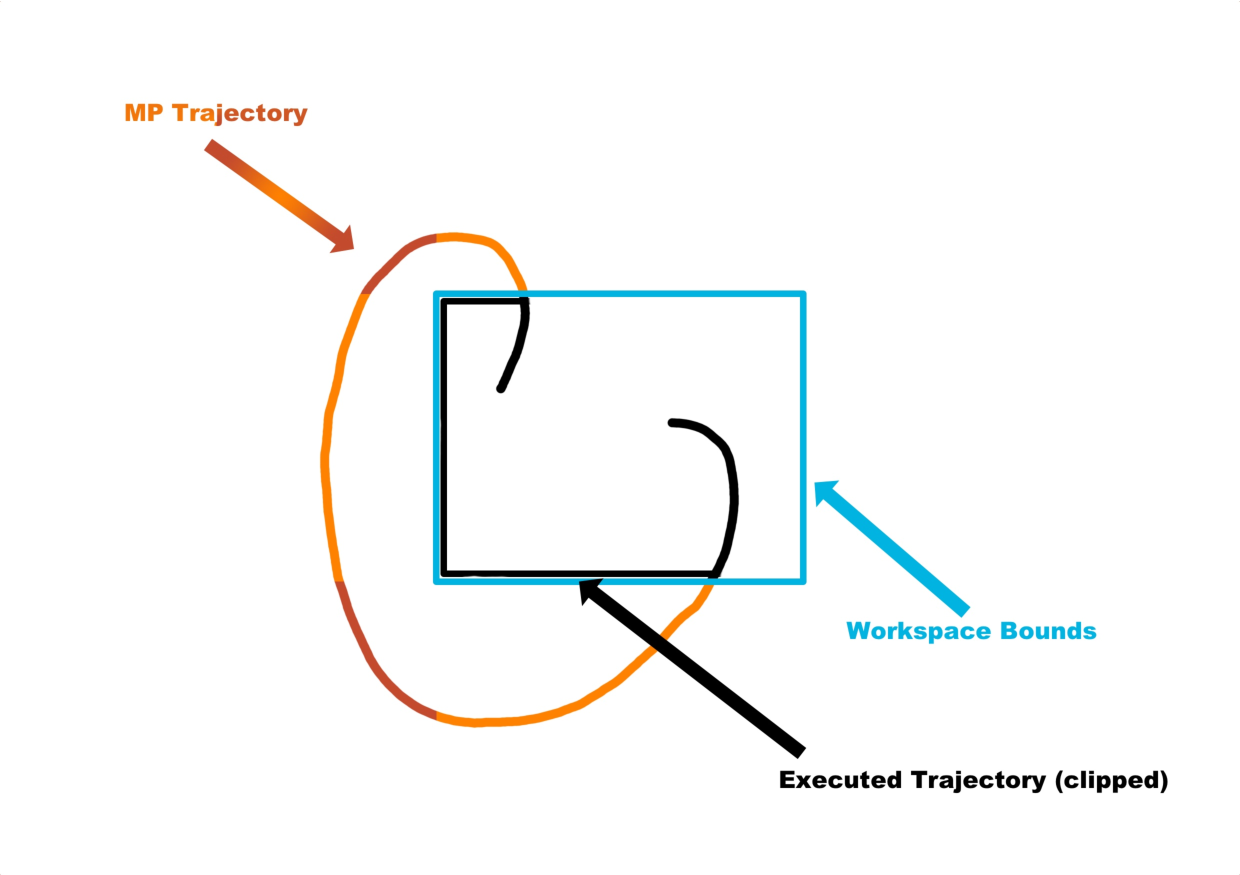
\includegraphics[width=\linewidth]{media/workspace_clipping.pdf}

		\end{column}
	\end{columns}
\end{frame}

\begin{frame}{Box Pushing --- Clipping}

	\begin{columns}
		\begin{column}{0.4\textwidth}
			\vspace{1cm}
			\begin{itemize}
				\item Clipping penality has a big effect on performance
				\item Every MP Env should have one
			\end{itemize}
		\end{column}
		\begin{column}{0.6\textwidth}
			\vspace{.2cm} \\
			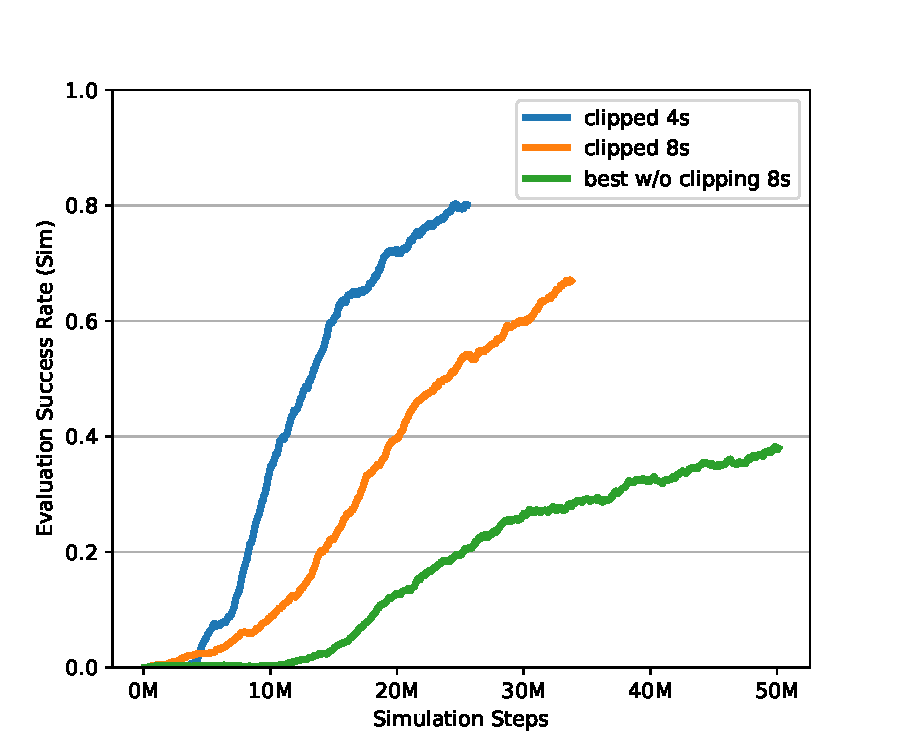
\includegraphics[width=\linewidth]{media/clipping_reward.pdf}

		\end{column}
	\end{columns}
\end{frame}

\begin{frame}{Box Pushing}

	\begin{columns}[t]
		\begin{column}{0.4\textwidth}
			\vspace{1cm}
			\begin{itemize}
				\item Goal: Use a finger to push a box to a target pose
				      \begin{itemize}
					      \item Random start pose
					      \item Fixed target pose
				      \end{itemize}
				\item Action space: 2D finger positions
				\item Observation:
				      \begin{itemize}
					      \item Finger position
					      \item Box quaternion + noisy position
				      \end{itemize}
				\item Success
				      \begin{itemize}
					      \item $\text{err}_{position} \leq 5 \text{cm}$
					      \item $\text{err}_{rotation} \leq 0.5 \text{rad}$
					      \item $\max_t(v_t) < v_\text{max}$
				      \end{itemize}
			\end{itemize}
			\vspace{1em}
		\end{column}
		\begin{column}{0.5\textwidth}
			\vspace{.5cm}
			\[
				\begin{aligned}
					\text{Reward} & := \textcolor{kit-blue100}{\text{Final Euclidean Distance}}                         \\
					              & +  \textcolor{kit-blue100}{\text{Final Rotational Distance}}                        \\
					              & +  \textcolor{kit-blue100}{\mathds{1} \left\{\text{success}\right\} }               \\
					              & -  \textcolor{kit-green100}{\max_t\  \text{step}(v_t)}                              \\
					              & -  \textcolor{kit-lila100}{\sum_t \left\Vert x_t - x_t^\text{clipped} \right\Vert } \\
					\\
					step(v) :=    & 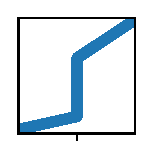
\includegraphics[scale=.4]{media/step.pdf}                                          \\
				\end{aligned}
			\]

		\end{column}
	\end{columns}
	\center
	Our reward includes \textcolor{kit-blue100}{sparse}, \textcolor{kit-green100}{non-markovian} and \textcolor{kit-lila100}{dense} components.
\end{frame}

\subsection{Making it work in Simulation}
\begin{frame}{Box Pushing --- In Simulation}

	\begin{columns}[t]
		\begin{column}{0.4\textwidth}
			\vspace{1cm}
			\begin{itemize}
				\item Box Pushing is \textbf{hard}.
				      \begin{itemize}
					      \item It took long to get $60-80$\% success in sim
					      \item 127 Sweeps so far, 2628 policies trained
					      \item $\approx 25-50\text{M}$ sim steps per policy
					      \item $\approx 60-120\text{K}$ 4s trajectories
				      \end{itemize}
				\item So many parameters:
				      \begin{itemize}
					      \item Reward coefficients
					      \item Maximum Speed $v_{\max}$
					      \item Amount of randomization
					      \item Episode Length
					      \item MP Parameters
					      \item TRPL Hyperparameters
				      \end{itemize}
			\end{itemize}
		\end{column}
		\begin{column}{0.5\textwidth}
			\vspace{.2cm} \\
			\center
			\includegraphics[width=.5\linewidth]{../fancy_gym/sweeps.pdf} \\

		\end{column}
	\end{columns}
\end{frame}

\subsection{Making it work on the real Robot}

\begin{frame}{Box Pushing --- Making it work on the real Robot}
	\begin{columns}
		\begin{column}{0.5\textwidth}
			\begin{itemize}
				\item No controller tracks perfectly
				\item The agent will \textbf{adapt} to the simulated controller under- or overshooting.
				\item Also the real robot trajectory has artifacts because of the 7DoF kinematics
				\item \textbf{Tuning for the real robot is crucial!}
			\end{itemize}
		\end{column}
		\begin{column}{0.5\textwidth}
			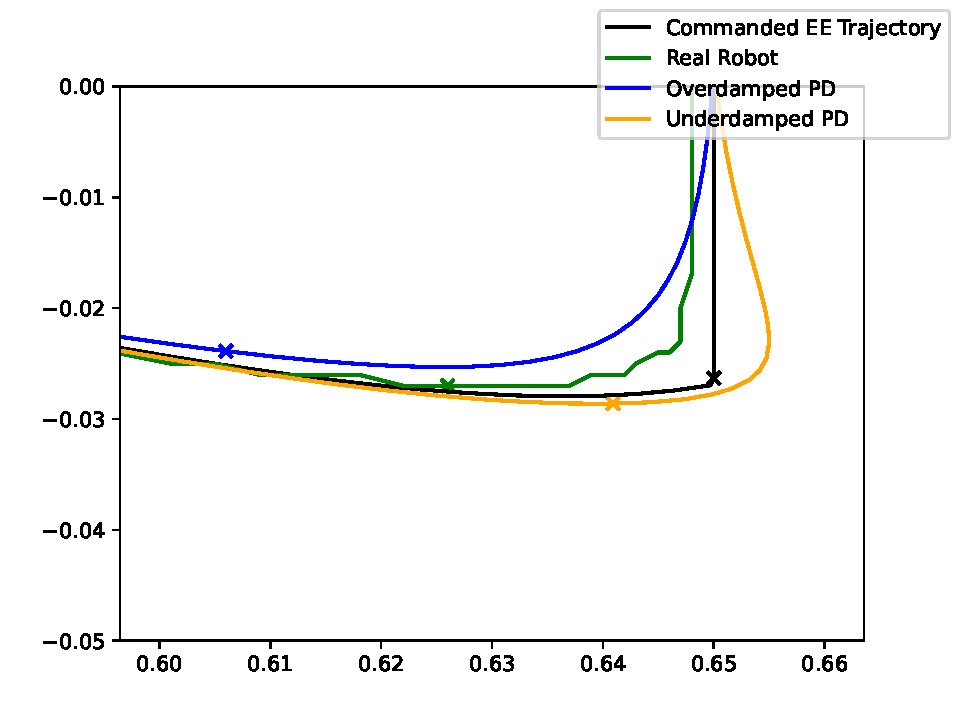
\includegraphics[width=\linewidth]{media/traj_error.pdf}
		\end{column}
	\end{columns}

\end{frame}
\begin{frame}{Box Pushing --- Making it work on the real Robot}
	\begin{columns}
		\begin{column}{0.5\textwidth}
			\begin{itemize}
				\item Our approach:
				      \begin{itemize}
					      \item Record real-robot executions
					      \item Optimize simulation PD parameters using bayesian optimization
					      \item Choose a lower/higher P-gain
					      \item Sample $Kp \sim \text{U}(Kp^-, Kp^+)$ during training
				      \end{itemize}

				      \[
					      \min_{kp, kd, mass} \sum_t \left\Vert x_t^\text{real} - x_t^\text{sim}(kp, kd, mass) \right\Vert
				      \]
			\end{itemize}
		\end{column}

		\begin{column}{0.5\textwidth}
			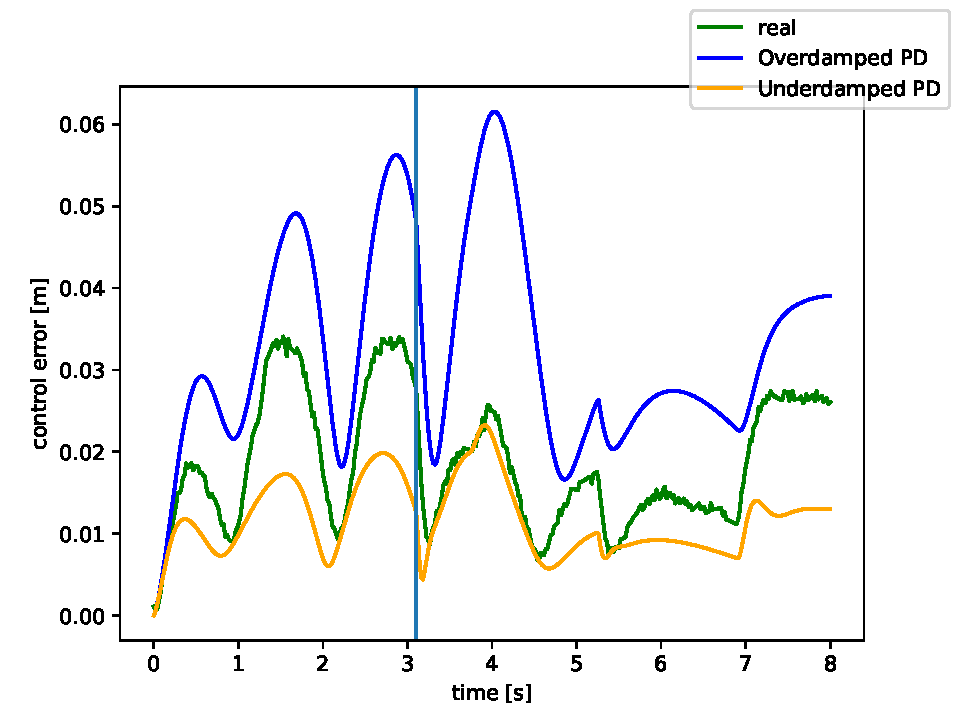
\includegraphics[width=\linewidth]{media/ctrl_error.pdf}\\
		\end{column}
	\end{columns}

\end{frame}

\section{Rollout Architecture}
\begin{frame}{Rollout Architecture}
	\begin{columns}
		\begin{column}{0.45\textwidth}
			\vspace{1cm}
			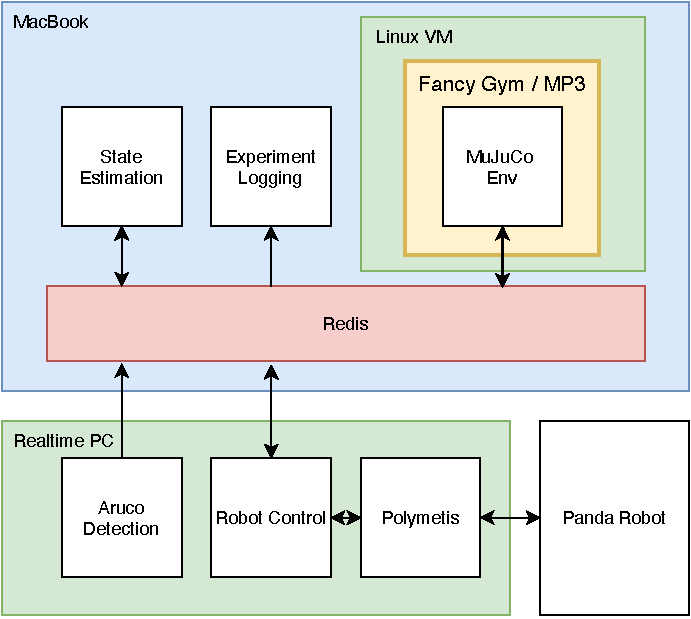
\includegraphics[width=\linewidth]{media/Architecture2.pdf}

		\end{column}
		\begin{column}{0.35\textwidth}
			\vspace{1cm}
			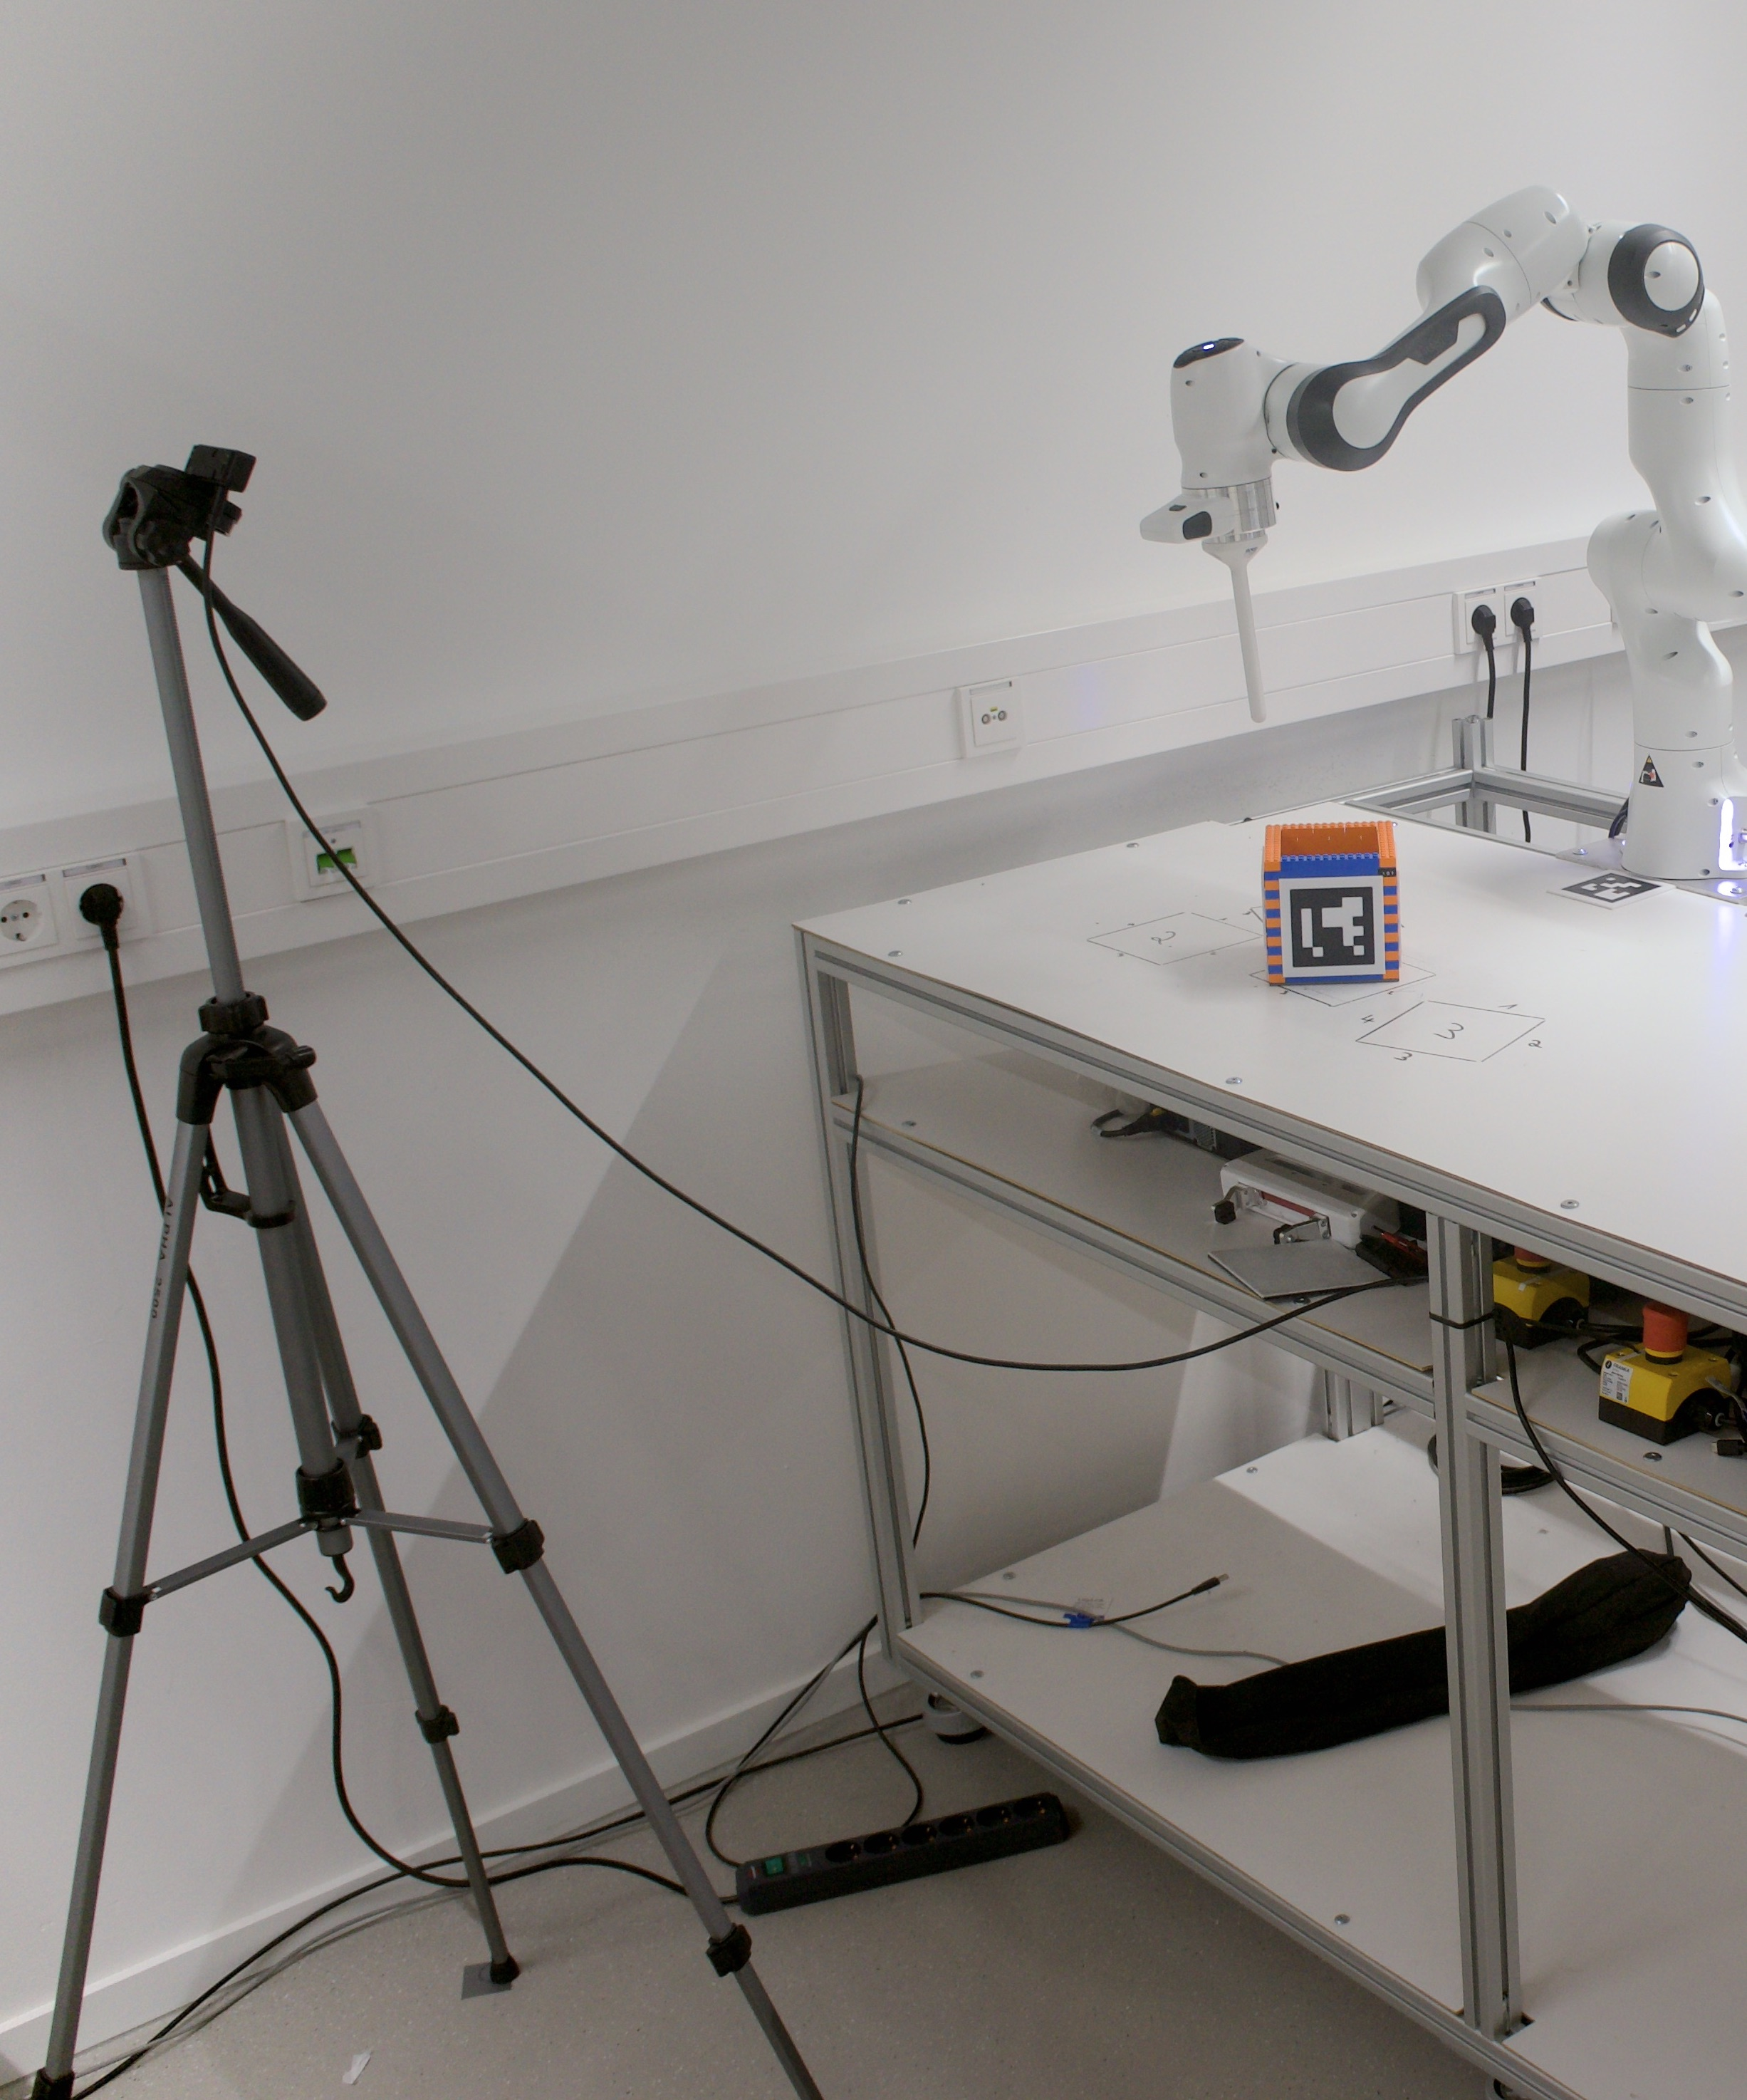
\includegraphics[width=\linewidth]{media/labsetup2.jpg}

		\end{column}
	\end{columns}

\end{frame}


\backupend{}

\end{document}
